
Results are presented in causal chain order: variance distribution $\rightarrow$ selection signal $\rightarrow$ training gradient concentration.

\subsubsection{5.1 RQ1: Variance Distribution (h-e1) --- Gate Passed}

The binary execution reward variance distribution on MBPP is severely right-skewed, but a meaningful high-variance subset exists.

\textbf{Table 2: MBPP Pass Rate Distribution (374 problems, k=4, max\_new\_tokens=128)}

\begin{table}[htbp]
\centering
\resizebox{\columnwidth}{!}{%
\begin{tabular}{llll}
\toprule
Pass Rate (p\_i) & Count & Percentage & Variance (v\_i) \\
\midrule
0.00 (all-fail) & 343 & 91.7\% & 0.0000 \\
0.25 (1/4 pass) & 29 & 7.8\% & 0.1875 \\
0.50 (2/4 pass) & 0 & 0.0\% & 0.2500 \\
0.75 (3/4 pass) & 0 & 0.0\% & 0.1875 \\
1.00 (all-pass) & 2 & 0.5\% & 0.0000 \\
\bottomrule
\end{tabular}
}
\end{table}

Source: \texttt{h-e1/results/mbpp\textbackslash \_variance\textbackslash \_profile.json}, confirmed in \texttt{h-e1/04\textbackslash \_validation.md}.

29 problems satisfy v\_i > 0.1, exceeding the gate threshold of 15 (gate passed). No problems were observed at pass rates 0.50 or 0.75 --- a consequence of k=4 granularity combined with max\_new\_tokens=128 truncation. The 91.7\% per-problem all-fail rate under profiling substantially exceeds the 54.75\% all-fail component reported by Nie et al. [2026] under different generation conditions, suggesting that constrained generation parameters amplify practical gradient starvation.

The mean p\_i across all 374 problems is 0.035. The mean p\_i across the top-50 variance-selected problems is 0.225.

\begin{figure}[htbp]
\centering
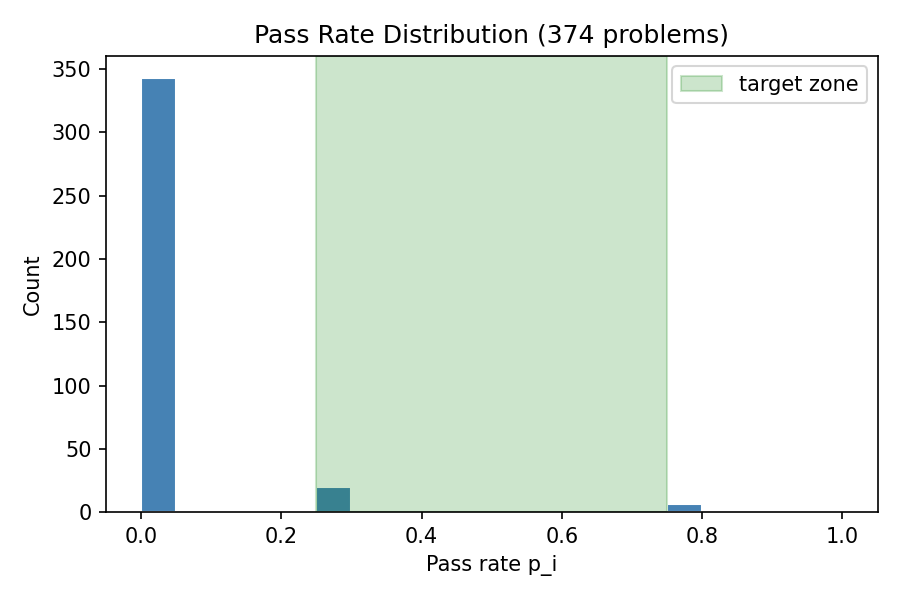
\includegraphics[width=\columnwidth]{figures/fig2_pass_rate_histogram.png}
\caption{Pass rate histogram for MBPP training problems (374 problems, k=4, max\_new\_tokens=128). The distribution is bimodal: 91.7\% at p\_i=0, 7.8\% at p\_i=0.25.}
\label{fig:fig2_pass_rate_histogram}
\end{figure}

\textit{Figure 1: Pass rate histogram for MBPP training problems (374 problems, k=4, max\_new\_tokens=128).}

\begin{figure}[htbp]
\centering
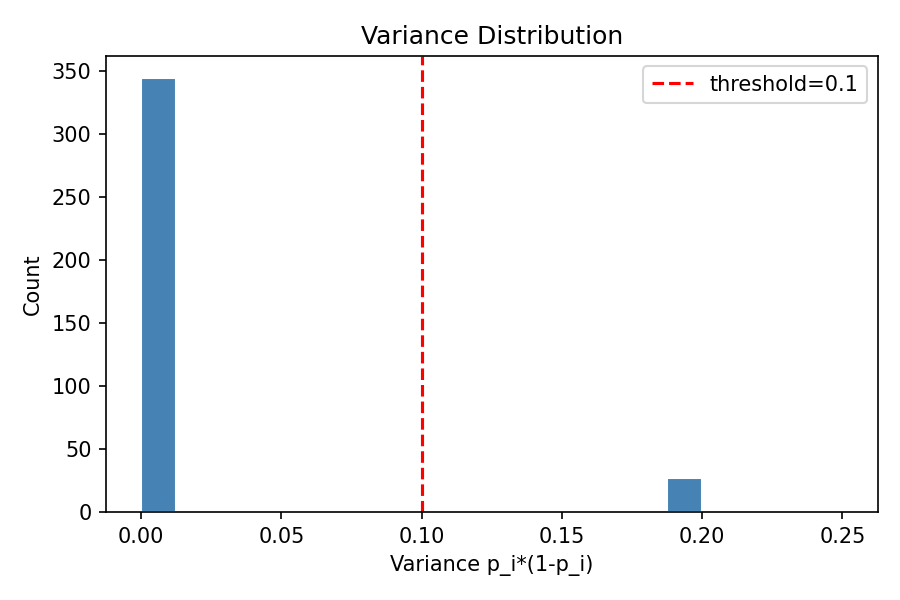
\includegraphics[width=\columnwidth]{figures/fig3_variance_histogram.png}
\caption{Variance histogram for MBPP training problems. 343 problems have v\_i=0; 29 have v\_i=0.1875. No intermediate levels exist under k=4 discrete sampling.}
\label{fig:fig3_variance_histogram}
\end{figure}

\textit{Figure 2: Variance distribution histogram. 343 problems cluster at v\_i=0; 29 problems at v\_i=0.1875.}

\textbf{Gate verdict (h-e1): Passed} --- existence of gradient-signal subset confirmed.

\subsubsection{5.2 RQ2: Selection Signal (h-m1) --- Gate Passed}

Variance-guided selection achieves 4.$24\times$ higher mean variance than random selection, with a highly significant difference.

\textbf{Table 3: Variance Selection Comparison}

\begin{table}[htbp]
\centering
\resizebox{\columnwidth}{!}{%
\begin{tabular}{lll}
\toprule
Metric & Variance-50 & Random-50 \\
\midrule
Mean variance & 0.1113 & 0.0262 \\
Ratio & 4.$24\times$ & 1.$0\times$ \\
Difference & 0.0850 & --- \\
Mann-Whitney U statistic & 1807.0 & --- \\
Mann-Whitney U p-value (one-sided) & 2.$22\times 10^{-6}$ & --- \\
\bottomrule
\end{tabular}
}
\end{table}

Source: \texttt{h-m1/results/comparison\textbackslash \_results.json}.

The Mann-Whitney U test (one-sided, alternative='greater') confirms that variance-50 problems have statistically higher variance than random-50 problems (p=2.$22\times 10^{-6}$ < 0.05). The empirical CDF of variance-50 lies entirely above that of random-50, confirming stochastic dominance.

The selection includes 21 zero-variance filler problems at the boundary (boundary\_gap=0), since only 29 problems have positive variance while the top-50 requires 50. Despite this, the overall distribution of the variance-selected subset differs dramatically from random selection.

\begin{figure}[htbp]
\centering
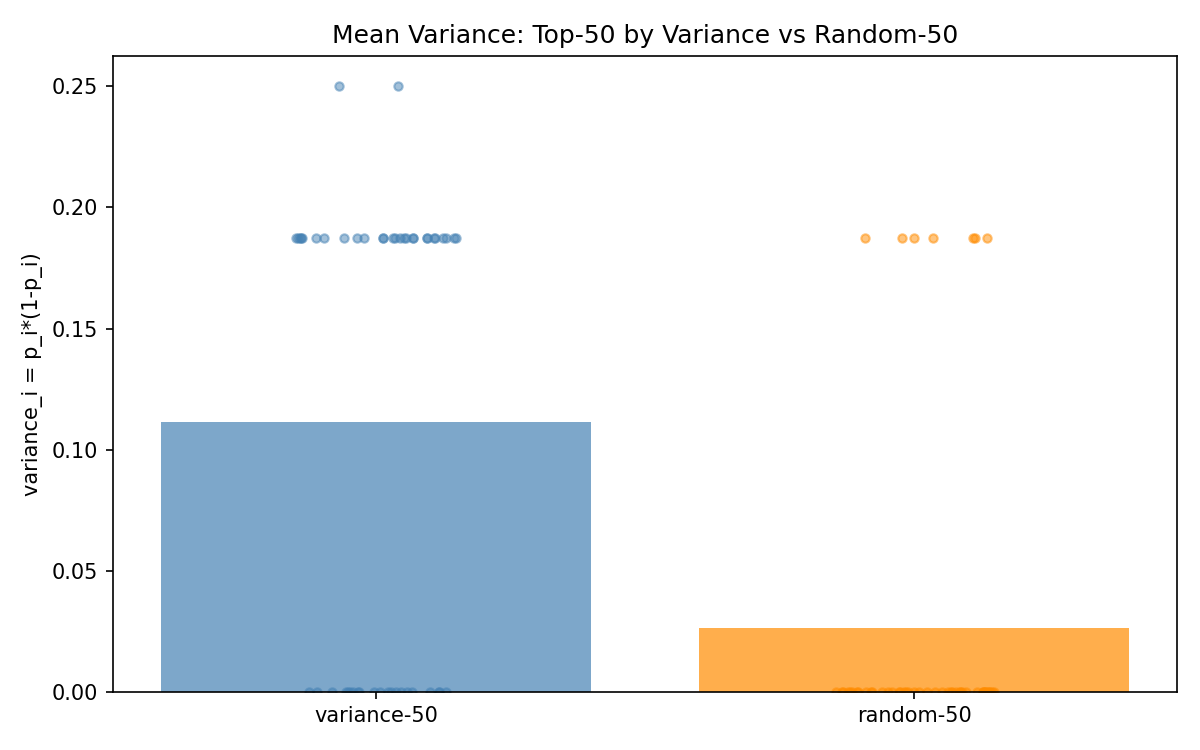
\includegraphics[width=\columnwidth]{figures/fig1_mean_comparison.png}
\caption{Mean variance comparison between variance-50 and random-50 selections, with individual data points shown. Variance-50 mean (0.1113) is 4.$24\times$ higher than random-50 mean (0.0262).}
\label{fig:fig1_mean_comparison}
\end{figure}

\textit{Figure 3: Mean variance comparison (variance-50 vs random-50) with individual data points.}

\begin{figure}[htbp]
\centering
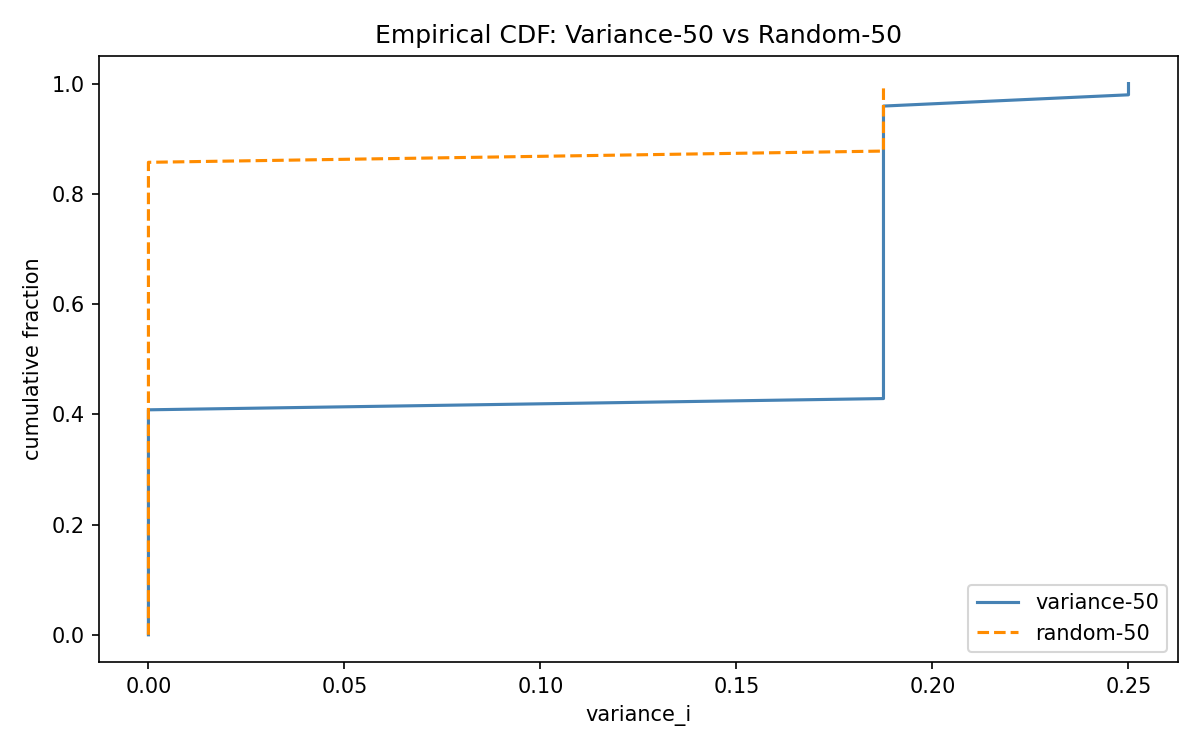
\includegraphics[width=\columnwidth]{figures/fig4_cdf.png}
\caption{Empirical CDF comparison: variance-50 lies entirely above random-50, confirming stochastic dominance.}
\label{fig:fig4_cdf}
\end{figure}

\textit{Figure 4: Empirical CDF of variance values for variance-50 and random-50. Variance-50 stochastically dominates random-50.}

\textbf{Gate verdict (h-m1): Passed} --- selection signal confirmed.

\subsubsection{5.3 RQ3: Gradient Concentration During Training (h-m2, h-m3) --- Gates Failed}

Both conditions show frac\_reward\_zero\_std=1.0 throughout all training steps in both experiments.

\textbf{h-m2 (50 steps, LR=$5\times 10^{-7})$:} Both variance-50 and random-50 maintained frac\_reward\_zero\_std=1.0 at every step. reward/mean=0.0, grad\_norm=0.0 throughout. TRL GRPOTrainer logged 13 generation-phase steps (due to off-policy replay). Total generation attempts: approximately 50 steps $\times$ 50 problems $\times$ 4 completions = 10,000, all returning reward=0.

\textbf{Table 4: H-M2 Gate Results (50 Steps)}

\begin{table*}[htbp]
\centering
\resizebox{\dimexpr 2\columnwidth+\columnsep\relax}{!}{%
\begin{tabular}{lllll}
\toprule
Checkpoint & frac\_reward\_zero\_std (variance-50) & frac\_reward\_zero\_std (random-50) & Gap & Gate pass \\
\midrule
Step 10 & 1.0000 & 1.0000 & 0.0000 & False \\
Step 20 & 1.0000 & 1.0000 & 0.0000 & False \\
Step 50 & 1.0000 & 1.0000 & 0.0000 & False \\
\bottomrule
\end{tabular}
}
\end{table*}

Source: \texttt{h-m2/results/gate\textbackslash \_results.json}.

\textbf{h-m3 (200 steps, LR=$1\times 10^{-6})$:} Cold-start persisted despite doubled learning rate and $4\times$ more training steps. frac\_reward\_zero\_std=1.0 throughout all 200 steps. Condition A (variance-50): 200 steps completed, max\_reward=0.0. Condition B (random-50): 200 steps completed, max\_reward=0.0. Total additional attempts: 200 steps $\times$ 50 problems $\times$ 4 completions = 40,000, all reward=0.

Source: \texttt{h-m3/results/gate\textbackslash \_results.json}, \texttt{h-m3/04\textbackslash \_validation.md}.

\textbf{Combined total: more than 50,000 generation attempts, zero reward across all conditions.}

The 4.$24\times$ selection signal from RQ2 is completely invisible during training. $\sigma =\sqrt(k(G-k))/G=0$ when k=0 for every problem --- cold-start nullifies any selection advantage before any gradient can be generated.

\begin{figure}[htbp]
\centering
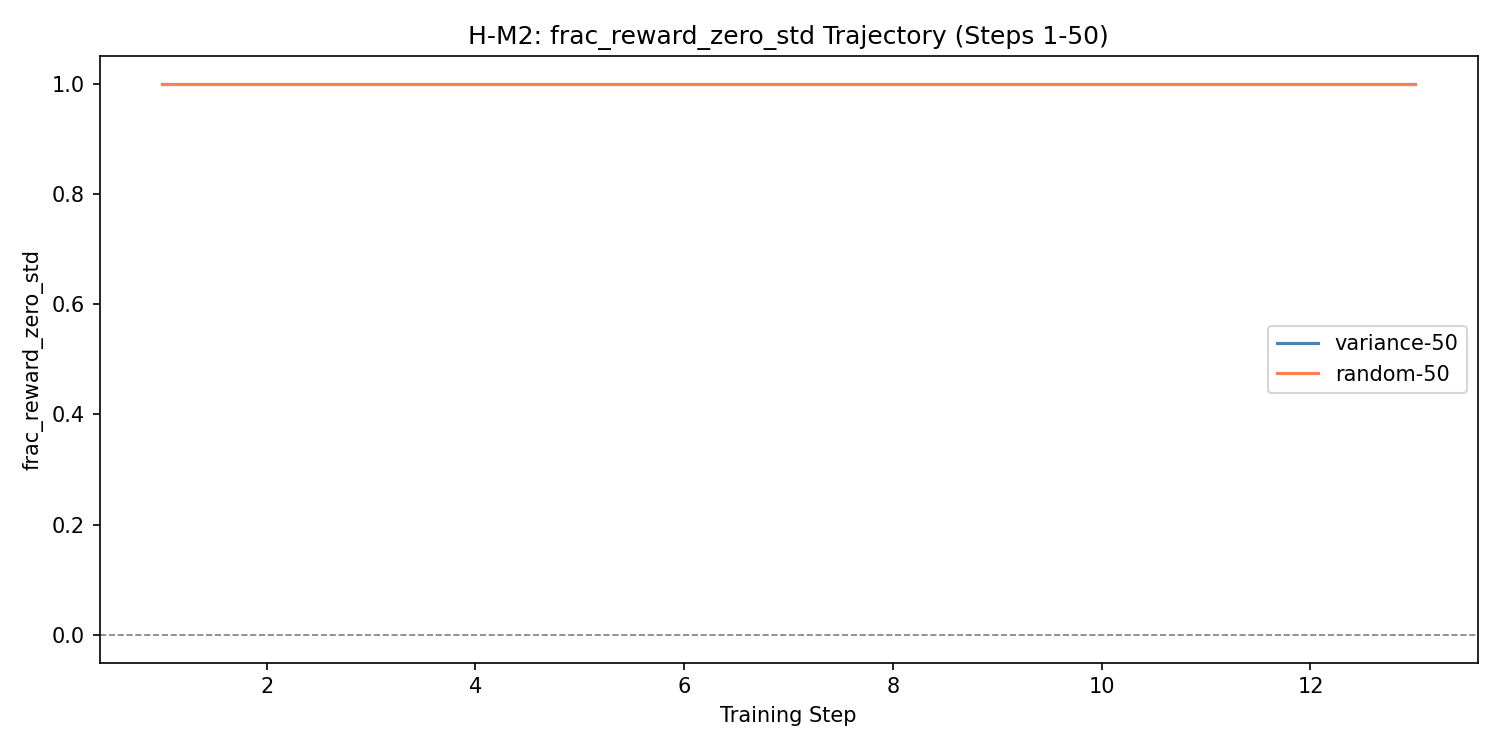
\includegraphics[width=\columnwidth]{figures/learning_curves.png}
\caption{Per-step frac\_reward\_zero\_std for variance-50 and random-50 conditions (h-m2, 50 steps). Both conditions are flat at 1.0 throughout, visually indistinguishable.}
\label{fig:learning_curves}
\end{figure}

\textit{Figure 5: frac\_reward\_zero\_std per training step (h-m2, 50 steps). Both conditions maintain 1.0 throughout.}

\textbf{Gate verdicts (h-m2, h-m3): Failed} --- mechanism Step 3 falsified under current parameters.

\textbf{HumanEval+ evaluation:} Not conducted. Cold-start prevented accumulation of any reward signal; no checkpoint was saved at step 50; evaluation was not possible.

